%!TEX TS-program = xelatex
%!TEX options = -aux-directory=Debug -shell-escape -file-line-error -interaction=nonstopmode -halt-on-error -synctex=1 "%DOC%"
\documentclass{article}
\input{LaTeX-Submodule/template.tex}

% Additional packages & macros
\usepackage[skip=8pt]{parskip}

% Header and footer
\newcommand{\unitName}{Systems Programming}
\newcommand{\unitTime}{Semester 2, 2023}
\newcommand{\unitCoordinator}{Dr Timothy Chappell}
\newcommand{\documentAuthors}{Tarang Janawalkar}

\fancyhead[L]{\unitName}
\fancyhead[R]{\leftmark}
\fancyfoot[C]{\thepage}

% Copyright
\usepackage[
    type={CC},
    modifier={by-nc-sa},
    version={4.0},
    imagewidth={5em},
    hyphenation={raggedright}
]{doclicense}

\date{}

\begin{document}
%
\begin{titlepage}
    \vspace*{\fill}
    \begin{center}
        \LARGE{\textbf{\unitName}} \\[0.1in]
        \normalsize{\unitTime} \\[0.2in]
        \normalsize\textit{\unitCoordinator} \\[0.2in]
        \documentAuthors
    \end{center}
    \vspace*{\fill}
    \doclicenseThis
    \thispagestyle{empty}
\end{titlepage}
\newpage
%
\tableofcontents
\newpage
%
\section{Operating Systems Overview}
An operating system is software that manages a computer's hardware.
It also provides a basis for application programs and acts as an
intermediary between the computer user and the computer hardware.
The purpose of an operating system is to:
\begin{itemize}
    \item execute user programs and make solving user problems easier
    \item make the computer system convenient to use
    \item use computer hardware in an efficient manner
\end{itemize}
\subsection{What Operating Systems Do}
A computer system is divided into four components:
\begin{itemize}
    \item Hardware that provides basic computing resources, i.e., the CPU, memory, and I/O devices
    \item An operating system which controls and coordinates the use of hardware for applications and users
    \item Application programs that define how system resources are used to solve user computing problems
    \item Users that make use of the computer system. This includes people, machines, or other computers
\end{itemize}
We can also view a computer system as consisting of hardware, software, and data.

This hierarchy of components is layered such that users cannot directly access the hardware.
As there are multiple different types of computer hardware, applications will typically rely on the operating system
to manage the use of computer hardware so that applications can designed to operate on any hardware. Due to this,
the operating system will typically restrict direct access to hardware resources.

The task of an operating system is to provide convenience, such that users do not have to worry about resource utilisation.
Depending on the type of user, a computer system will prioritise one of the following:
\begin{itemize}
    \item Shared computers such as mainframes or minicomputers are required to distribute resources to multiple users.
    \item Dedicated systems such as workstations have dedicated resources for a single user, but will frequently use shared resources (such as CPU cores or memory) from servers.
    \item Handheld devices (such as phones, tablets, and laptops) are resource poor in comparison to desktop devices, and are optimised for usability, portability, and battery life.
    \item Embedded devices often have little or no user interface, but access computing resources via alternate means, such as sensors in vehicles.
\end{itemize}
\begin{definition}[Operating System]
    An Operating System (OS) is a \textbf{resource allocator} that manages all resources in a computer system
    that resolves conflicting requests of resources by efficiently and fairly distributing resources.

    An OS is also a \textbf{control program} that controls the execution of programs to prevent errors and improper use of it's system.
    The OS acts as a security layer between applications, such that one application cannot interfere with another, or bring down the entire system.

    An OS must therefore be robust and reliable\footnote{This is far less onerous than requiring \underline{all applications} to be error-free.}.
\end{definition}
A more common definition is that the OS is the one program that runs at all times on the computer, which is known as the \textbf{kernel},
and is the core of the operating system. Everything else is either a \textbf{system program}, which are associated with the OS, or an \textbf{application program}.
\subsection{Computer System Organisation}
\subsubsection{Device Controllers}
A computer system consists of one or more CPUs and a number of \textbf{device controllers}
connected through a common \textbf{bus} that provides access between components and shared memory.
This bus is responsible for concurrent communication between the CPU and other devices.

Each device controller is responsible for a specific type of device, and depending on the device,
may have more than one device attached. A device controller maintains a \textbf{local buffer}
and a set of \textbf{special-purpose registers}.
The device controller is responsible for moving data between the device and its local buffer,
which is then moved to/from main memory by the CPU.

Typically, operating systems have a \textbf{device driver} for each device controller. This
device driver understands the device controller and provides a uniform interface to the rest of the operating system.

Device controllers inform the CPU that they have finished their operation by causing an \textbf{interrupt}.
\subsection{Computer Operation}
Consider a typical computer operation of performing I/O.
\begin{enumerate}
    \item To start the operation, the device driver loads the appropriate registers within the device controller.
    \item The device controller examines the contents of these registers to determine what actions to take.
    \item The device controller will then start the transfer of data from the device to its local buffer.
    \item Once the transfer is complete, the device controller informs the device driver that it has finished its operation.
    \item The device driver then gives control back to the operating system, through an interrupt.
\end{enumerate}
\subsection{Interrupts}
Operating systems are \textbf{interrupt driven}, and will respond to events as they occur.

Interrupts \textbf{transfer control} to an \textbf{interrupt service routine} (ISR) through the
\textbf{interrupt vector}, which contains the address of all service routines, stored in low memory for
quick access.
A serice routine is simply a function, or piece of code, that is executed when an interrupt occurs.

Hardware may trigger an interrupt at any time by sending a signal to the CPU, usually through the system bus.

When an interrupt occurs, the CPU halts it's current execution and the interrupt architecture saves the address
of the interrupted instruction, so that it can be resumed once the ISR has finished. The CPU then jumps to a
fixed location in memory, which is the starting address of the ISR.

The interrupt architecture must also save the state information of the interrupted process, so that it can be
restored once the ISR has finished.
\subsubsection{Implementation}
The basic interrupt mechanism is described below.

The CPU has an \textbf{interrupt-request line} that the CPU sense after executing
every instruction. When the CPU detects that a controller has \textit{asserted} a signal
onto this line, it reads the interrupt number and jumps to the corresponding \textbf{interrupt-handler routine}.

The interrupt handler:
\begin{itemize}
    \item saves any state it will change during its operation
    \item determines the cause of the interrupt
    \item performs the necessary processing
    \item restores the saved state
    \item executes a \textbf{return from interrupt} instruction, which returns the CPU to the execution state,
          prior to the interrupt
\end{itemize}
A device controller \textbf{raises} an interrupt by asserting a signal on the interrupt-request line,
and the CPU \textbf{catches} the interrupt and \textbf{dispatches} it to the interrupt handler, which
then \textbf{clears} the interrupt by servicing the device.
\subsubsection{Types of Interrupts}
A \textbf{trap} or \textbf{exception} is a software-generated interrupt caused by an error or a user request,
and is often used to communicate with the operating system. Software can trigger an interrupt through a special
operation called a \textbf{system call} (or monitor call).

An operating system also makes a distinction between the following types of interrupts:
\begin{itemize}
    \item For a \textbf{polled} interrupt, the operating system periodically queries a queue of interrupts, to see if one needs to be serviced.
    \item In a \textbf{vectored} interrupt system, the interrupt vector table will interrupt the CPU to service the necessary interrupt.
\end{itemize}
\subsection{Storage Structure}
\subsubsection{Main Memory}
The CPU can only load instructions from memory, and therefore programs must first be
loaded into memory before they can be executed. Computers run most of their programs
from rewritable memory, called \textbf{main memory} (or \textbf{random-access memory} (RAM)), which
means that it can both read and write to any location in memory.

Main memory is \textbf{volatile} and will lose its content when power is lost.
\subsubsection{Registers}
All forms of memory provide an array of \textbf{bytes} (or words) that can be individually accessed by
a \textbf{memory address}. The CPU interacts with these memory locations through \textbf{load} or \textbf{store}
instructions.
\begin{itemize}
    \item A \textbf{load} instruction moves data from main memory into an internal register in the CPU
    \item A \textbf{store} instruction moves data from an internal register in the CPU to main memory
\end{itemize}
The operating system preserves the state of the CPU through \textbf{registers}.
Registers can store data within the CPU, and are the fastest form of memory available to the CPU.

Registers are often used to carry out operations such as addition, where the two operands
are stored in two registers, before their sum can be computed and saved to another register or in memory.

The CPU also uses registers for storing other information such as the status of an operation,
and the program counter, which is the address of the next instruction to be executed.
\subsubsection{Cache Management}
Caching is an important principle in computer systems, and is used to improve performance
at many levels of a computer system. Caching refers to the temporary copying of data from a
slower storage system into a faster storage system, where it can be accessed more quickly.

When some piece of information is required, we first check whether
a copy of that data is in the cache.
\begin{itemize}
    \item If so, we use the information directly from the cache
    \item If not, we use the information from the source, while placing a copy of that data into the cache, under
          the assumption that it will be needed again soon
\end{itemize}
Internal programmable registers provide high-speed cache for main memory. The programmer (or compiler)
implements register allocation and replacement algorithms to decide which information is kept in
registers and which is kept in main memory.

Other caches are implemented in hardware. For example, most systems have an \textbf{instruction cache}
to hold instructions expected to be executed next. Without this cache, the CPU would have to wait
several cycles for the instruction to be fetched from main memory. For similar reasons, most
systems have one or more high-speed data caches in the memory hierarchy.

Because caches have limited size, \textbf{cache management} is an important design problem.
Careful selection of cache size and of a replacement policy can significantly improve performance.

The movement of information between levels of a storage hierarchy may be either \textbf{explicit} or \textbf{implicit}.
For instance, data transfer from cache to the CPU and registers is usually a hardware function, with no operating system intervention.
In contrast, transfer of data from disk to memory is usually controlled by the operating system.
\paragraph{An Example}

Consider the following example where an integer \(A\) is to be incremented by 1, and is located in file \(B\) which resides on hard disk.
\begin{enumerate}
    \item The operating system loads the file \(B\) from disk into main memory.
    \item The operating system then load the integer \(A\) from main memory into the cache of an internal register.
    \item The CPU performs the increment operation on the internal register.
    \item The operating system then updates value of \(A\) from internal memory to the file \(B\) in main memory.
    \item The operating system then writes the updated value of \(B\) back to disk.
\end{enumerate}
\paragraph{Implications of Various Environments}

In a single processor system, where only one process executes at a time,
this hierarchy poses no difficulties, as access to the integer \(A\) will
always be to the copy at the \textbf{highest level} of the hierarchy.

In a \textbf{multitasking environment}, where multiple processes execute concurrently,
extreme care must be taken to ensure that, if two or more processes are accessing the same data,
then each process must access the \textbf{most recently updated} copy of the data.

Furthermore, in a \textbf{multiprocessor environment}, each CPU also contains a local cache.
In such an environment, a copy of data may exist simultaneously
in several caches. As these CPUs can execute in parallel, we must ensure that
an update to data is propagated to all copies of the data in all caches.

This is known as \textbf{cache coherency}, and is usually a hardware level problem.
\subsubsection{Secondary Storage}
Systems with a \textbf{von Neumann architecture} fetch instructions from memory and
store them in the \textbf{instruction register}. When this instruction is decoded,
it may require addition operands to be fetched from memory, and stored into internal
registers.

Ideally, we want programs and data to be stored in main memory permanently, to allow
for fast access. However, main memory is usually too small to store all necessary
programs and data permanently, and volatile.

Thus, most computer systems provide \textbf{secondary storage} as an extension of
main memory. Secondary storage is nonvolatile and is used to store large amounts
of data permanently. It is usually much slower than main memory.

Programs are stored in secondary storage until they are loaded into memory.
The most common forms of secondary storage are \textbf{hard-disk drives} (HDDs) and
\textbf{nonvolatile memory} (NVM) \textbf{devices}.
\subsubsection{Tertiary Storage}
Large storage capacities can also be achieved through \textbf{tertiary storage}, which
is used for data that is not frequently accessed, such as in archival storage, or
for backup. Examples of this type of storage includes \textbf{magnetic tape} and \textbf{optical disk} storage.
\subsubsection{Summary}
A summary of the storage hierarchy is shown below.
\begin{figure}[H]
    \centering
    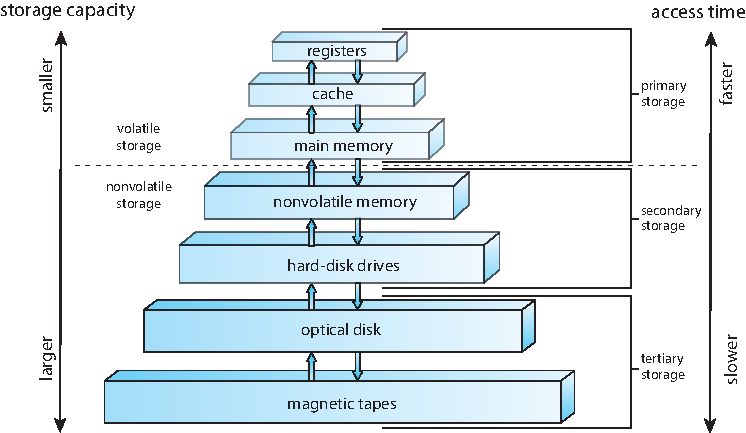
\includegraphics[height = 6cm]{figures/storage_hierarchy.pdf}
    % \caption{} % \label{}
\end{figure}
From here onwards, the term \textbf{memory} will be used to refer to volatile storage,
while \textbf{nonvolatile storage} (NVS) will be used to refer to nonvolatile storage.

The design of a complete storage system must balance,
\begin{itemize}
    \item Cost: NVS is cheaper than memory
    \item Performance: memory is faster than NVS
    \item Volatility: memory loses its contents when power is lost
\end{itemize}
\subsection{I/O Structure}
I/O is structured in one of two ways:
\begin{enumerate}
    \item After I/O starts, control returns to the user program only upon I/O completion.
          \begin{itemize}
              \item \textbf{Wait instructions} idle the CPU until the next interrupt
              \item At most one I/O request is outstanding at a time, and no simultaneous I/O processing is possible
          \end{itemize}
    \item After I/O starts, control returns to the user program without waiting for I/O completion.
          \begin{itemize}
              \item \textbf{System calls} request the OS to allow the user to wait for I/O completion
              \item A \textbf{device-state table} contains entries for each I/O device, indicating its type, address, and state
              \item The OS indexes into this table to determine the device status and modifies the table entry to include interrupt information
          \end{itemize}
\end{enumerate}
\subsubsection{Direct Memory Access}
The form of interrupt-driven I/O described above is sufficient for
moving small amounts of data, but can produce high \textbf{overhead} when used for bulk data transfer.

To solve this problem, \textbf{direct memory access} (DMA) is used. This allows device controllers to transfer
entire blocks of data directly to or from the device and main memory, without CPU intervention.
Only one interrupt is generated per block, to indicate the operation has completed, rather than one interrupt per byte.
\begin{figure}[H]
    \centering
    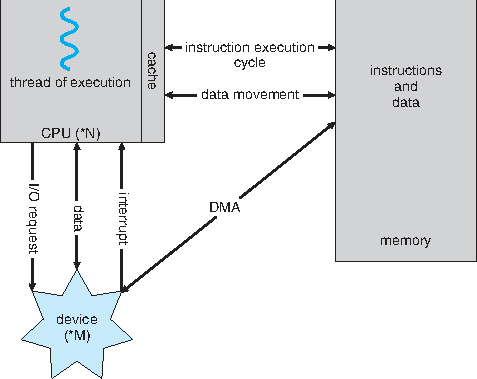
\includegraphics[height = 6cm]{figures/dma.pdf}
    % \caption{} % \label{}
\end{figure}
While the device controller is performing these operations, the CPU is idle, and can be used by another process.
\subsection{Computer-System Architecture}

\begin{tcolorboxlarge}[title={Definitions}, parbox=false]
    This section will use the following definitions:
    \begin{description}
        \item[Core] The basic computation unit of the CPU
        \item[CPU] The hardware that executes instructions
        \item[Processor] A physical chip that contains one or more CPUs
        \item[Multicore] Multiple cores on the same CPU
        \item[Multiprocessor] Multiple processors
    \end{description}
\end{tcolorboxlarge}

\subsubsection{Single-Processor Systems}
A single processor system is one which contains a single general purpose CPU with a single processing core.

Older computer systems used a single processor containing one CPU with a single processing core.
The \textbf{core} is the component that executes instructions and accesses registers for storing data locally.
The \textbf{CPU} is capable of executing a \textbf{general-purpose} instruction set, including instructions from
processes.

These systems also have other \textbf{special-purpose} processors such as device-specific processors for
disk, keyboard, and graphics controllers. These processors run a limited instruction set and
cannot run processes.

Sometimes these processors are managed by the OS, which sends them
information about the next task and monitors their status.

In other systems, special-purpose processors are low-level components built into the hardware.
The OS cannot communicate with these processors, as they execute jobs autonomously.
\subsubsection{Multiprocessor Systems}
Multiprocessor systems (or \textbf{parallel (tightly-coupled) systems}),
are systems with two or more processors.
\begin{figure}[H]
    \centering
    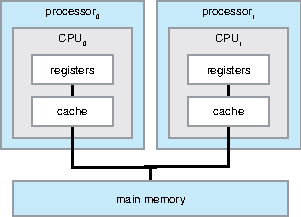
\includegraphics[height = 6cm]{figures/multiprocessing.pdf}
    % \caption{} % \label{}
\end{figure}
Multiprocessor systems have several advantages over
single processor systems:
\begin{itemize}
    \item \textbf{Increased throughput}: More work can be accomplished in less time
    \item \textbf{Economy of scale}: Multiprocessor systems are cheaper than equivalent multiple single processor systems
    \item \textbf{Increased reliability}: Graceful degradation or fault tolerance --- if one CPU fails, the system can continue to operate
\end{itemize}
There are two types of multiprocessor systems:
\begin{itemize}
    \item \textbf{Asymmetric multiprocessing}: Each processor is assigned a specific task, such as I/O or process scheduling
    \item \textbf{Symmetric multiprocessing}: Each processor performs all tasks, including OS activities
\end{itemize}

\begin{tcolorboxlarge}[title={Symmetric Multiprocessing}, parbox=false]
    The most common multiprocessor systems use symmetric multiprocessing (SMP),
    where each CPU performs all tasks, including operating system functions and user
    processes. Each CPU has its own registers and cache, but all processors share
    physical memory over the \textbf{same bus}.

    The benefit of this model is that many processes can be run \textbf{simultaneously},
    without performance degradation. However, since CPUs are separate, one
    may be idle which another is busy, resulting in inefficiencies.

    One solution to this problem is to share certain \textbf{data structures} between processors.
    This will allow processors and resources (such as memory) to be shared
    dynamically amongst processors, reducing workload variation between processors.

    Such systems must properly \textbf{schedule} and \textbf{synchronise} access to shared resources,
    to avoid conflicts between processors.
\end{tcolorboxlarge}

\begin{tcolorboxlarge}[title={Multicore Systems}, parbox=false]
    Multicore systems are systems with multiple computing cores on the same chip (processor).
    \begin{figure}[H]
        \centering
        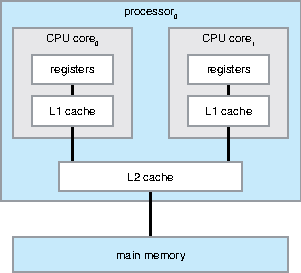
\includegraphics[height = 6cm]{figures/multicore.pdf}
        % \caption{} % \label{}
    \end{figure}
    Multicore systems:
    \begin{itemize}
        \item are more efficient than systems with multiple chips with single cores,
            because on-chip communication is faster than between-chip communication.
        \item use significantly less power than multiple single core chips.
    \end{itemize}
    Each core has its own local cache, known as \textbf{level-1}, or \textbf{L1 cache}.
    In addition to this, each core shares a \textbf{level-2}, or \textbf{L2 cache}, that is local to the chip.
    Lower levels of cache are generally smaller, but have faster access times than higher level shared caches.

    A multicore processor with \(N\) cores appears to the operating system as \(N\) standard CPUs. This
    requires operating system designers and application programmers to make efficient use of these additional
    processing cores.
\end{tcolorboxlarge}

\begin{tcolorboxlarge}[title={Non-Uniform Memory Access Multiprocessing Systems}, parbox=false]
    While adding additional CPUs to multiprocessor systems increases computing power, contention for
    the system bus creates a bottleneck and limits performance. An alternative approach is to provide
    each CPU (or groups of CPUs) with its own \textbf{local memory} that is accessed via a small but fast, local bus.
    These CPUs are connected by a \textbf{shared system interconnect}, so that all CPUs share one
    physical address space.

    This is known as a \textbf{non-uniform memory access} (NUMA) architecture.
    \begin{figure}[H]
        \centering
        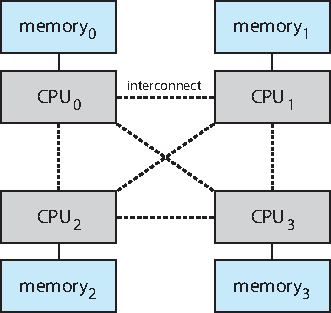
\includegraphics[height = 6cm]{figures/numa.pdf}
        % \caption{} % \label{}
    \end{figure}
    The advantages and disadvantages of NUMA multiprocessing architectures are as follows:
    \begin{itemize}
        \item CPUs have fast access to local memory and require no contention over the system interconnect
        \item NUMA can be scaled more effectively as more CPUs are added
        \item There is increased \textbf{latency} when accessing \textbf{remote memory} across the system interconnect
    \end{itemize}
    Due to their excellent scalability, NUMA systems are very popular on servers and high-performance computing systems.
\end{tcolorboxlarge}

\begin{tcolorboxlarge}[title={Blade Servers}, parbox=false]
Blade servers are systems in which multiple processor boards, I/O boards, and \linebreak networking boards are
placed in the same chassis. These servers consist of multiple independent multiprocessor systems,
that runs its own operating system.
\end{tcolorboxlarge}

\subsubsection{Clustered Systems}
Clustered systems are another type of multiprocessor system that are composed of two or more
individual systems, called \textbf{nodes}. Each system is typically a multicore system, and
the system is \textbf{loosely coupled}. Clustered computers share storage via a \textbf{storage-area network} (SAN)
and are usually connected via a \textbf{local-area network} (LAN).
\begin{figure}[H]
    \centering
    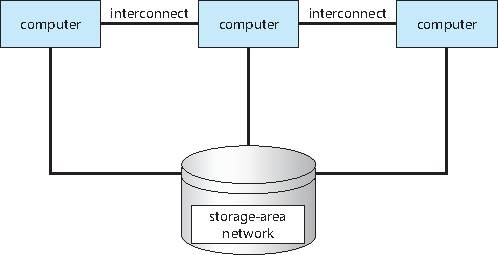
\includegraphics[height = 6cm]{figures/clustered_system.pdf}
    % \caption{} % \label{}
\end{figure}

\begin{tcolorboxlarge}[title={High-Availability Service}, parbox=false]
    The purpose of a clustered system is to provide a \textbf{high availability service}, that is,
    the ability to operate even if one or more nodes fail. This is achieved by adding a level of redundancy in
    the system. In this system, a layer of cluster software runs on the cluster nodes to monitor one or more
    nodes, such that if the monitored machine fails, the monitoring machine can take ownership of its resources.

    The ability to continue providing service proportional to the level of surviving hardware is called
    \textbf{graceful degradation}. Some systems are called \textbf{fault tolerant} if they can suffer
    a failure of a single component and still continue operation. Fault tolerance requires a
    mechanism to allow the failure to be detected, diagnosed, and corrected.

    Clustering can be structured asymmetrically or symmetrically:
    \begin{itemize}
        \item \textbf{Asymmetric clustering} has one machine in \textbf{hot-standby mode},
        while the other runs applications. The hot-standby host machine monitors the active server,
        so that if it fails, it will become the active server.
        \item \textbf{Symmetric clustering} has multiple hosts running applications, while monitoring each other.
        This structure is more efficient as it uses all available hardware, but only if more than one
        application is running.
    \end{itemize}
\end{tcolorboxlarge}

\begin{tcolorboxlarge}[title={High-Performance Computing}, parbox=false]
    As a cluster consists of several computer systems connected via a network, clusters
    can also provide \textbf{high-performance computing} (HPC) environments.
    Such systems supply significantly greater computational power because they can run applications
    concurrently on several computers.

    This is primarily useful for applications that utilise
    \textbf{parallelisation}, which is the process of breaking down a large task into smaller
    components that run on individual cores in a computer. These tasks are designed to then be
    recombined to produce the final result.
\end{tcolorboxlarge}

\begin{tcolorboxlarge}[title={Parallel Clustering}, parbox=false]
    Parallel clusters allow multiple hosts to access the same data on a shared storage over
    a \textbf{wide-area network} (WAN). Such systems require specialised versions
    of software that can support simultaneous data access by multiple hosts, to ensure
    that no conflicting operations occur. This function, commonly known as a
    \textbf{distributed lock manager} (DLM), is included in some cluster technologies.
\end{tcolorboxlarge}
\subsection{Operating System Operations}
\subsubsection{Computer Startup}
When a computer is turned on or rebooted, the first program it runs is a \textbf{bootstrap program} (\textbf{firmware}), which
then loads the operating system. This program is stored in \textbf{read only memory} (ROM)
or \textbf{electrically erasable programmable read only memory} (EEPROM).
This storage is infrequently written to and is nonvolatile.

This program will search for an operating system kernel within all connected hard disks, optical drives, or USBs, and load the first one it finds into memory.
The order in which this search is conducted is known as the \textbf{boot sequence}, and can be configured in the \textbf{basic input/output system} (BIOS).

Some services are provided outside of the kernel, by system programs, that are loaded into memory at boot time to become \textbf{system daemons},
which run while the kernel is running. On Linux, the first system program is ``\mintinline{text}|systemd|'', and it starts many other daemons.

Once this is completed, the system is fully booted, and waits for some event to occur. As discussed earlier, events are signalled
via interrupts.
\subsubsection{Multiprogramming}
Users of a system typically want to run multiple programs at the same time, rather than having one program keeping the CPU or I/O devices busy at all times.
\textbf{Multiprogramming} allows an operating system to increase CPU utilisation, and satisfy user requirements,
by organising jobs (code and data) such that the CPU always has one to execute.
In such a system, a program in execution is called a \textbf{process}.

The operating system keeps a subset of processes in memory, where the CPU executes processes one at a time, switching between processes
when the current process no longer requires the CPU or is waiting for I/O. This ensures the CPU is never idle as long as there are processes to execute.
This is known as \textbf{process scheduling}.
\subsubsection{Multitasking}
Multitasking (or \textbf{timesharing}) is a logical extension of multiprogramming, in which a CPU switches between multiple processes
frequently, providing the illusion that multiple processes are executing simultaneously.
For instance, the time a user takes to type a command or click a mouse is incredibly slow for a computer,
and hence the CPU may switch to another process while waiting for the user to provide input.

Multitasked systems require additional considerations:
\begin{itemize}
    \item \textbf{Interactive} systems require fast \textbf{response times} (less than 1s), so that users do not have to wait for long periods of time.
    \item Having several processes in memory requires \textbf{memory management}.
    \item If several processes are ready to be executed, \textbf{CPU scheduling} is required to decide which process to execute next.
    \item If multiple processes are executing concurrently, \textbf{process synchronisation} is required to ensure that processes do not interfere with each other.
\end{itemize}
For processes that are larger than \textbf{physical memory}, \textbf{virtual memory} may be used to execute processes that are stored partially in memory.
This arrangement of memories addresses memory usage constraints.

\emph{Both multiprogramming and multitasking systems must provide a \textbf{file system} to allow processes to access data stored on secondary storage.
In addition to this, they must \textbf{protect resources} from inappropriate use, provide mechanisms to process \textbf{synchronisation and communication}, and
ensure that processes do not get stuck in a \textbf{deadlock}.}
\subsection{Dual-Mode Operation}
As the operating system and users share hardware and software resources, the operating system must ensure that
malicious programs cannot cause other programs (or the operating system itself) to execute incorrectly.
To distinguish between the execution of operating system code and user-defined code, we can use
\textbf{dual-mode} operation:
\begin{itemize}
    \item \textbf{User mode} --- used for executing user-defined code, and restricts direct access to hardware and special instructions.
    \item \textbf{Kernel mode} --- used for executing operating system code, and allows direct access to hardware and all privileged instructions.
\end{itemize}
A \textbf{mode bit} is used to indicate the current mode of operation; 0, when the system is in kernel mode, and 1, when the system is in user mode.
At system boot time, hardware starts in kernel mode, and the operating system (when it is loaded), starts user applications in user mode.

When a trap or interrupt occurs, the hardware switches from user mode to kernel mode, and always switches to user mode \textit{before}
returning control to the user program.

This also allows us to designate certain machine instructions as \textbf{privileged instructions}, which can only be executed in kernel mode.
For example, the instruction to switch from user mode to kernel mode is a privileged instruction.
\subsection{Multi-Mode Operation}
The dual-mode concept can be extended to include multiple modes of operation, where each mode has a different level of privilege.
One such example of this is with CPUs that support virtualisation, where a separate mode is used to indicate when the \textbf{virtual machine manager} (VMM)
is in control of the system.
\subsection{Timers}
To ensure that the operating system maintains control over the CPU, a \textbf{timer} is used to prevent a user program from running indefinitely.
\begin{itemize}
    \item The operating system configures a timer to interrupt the CPU after a specific period of time, before transferring control to the user
    \item The timer is decremented for every clock tick
    \item An interrupt is generated when the timer reaches 0
    \item The operating system decides whether to regain control of the CPU, or allow the program to continue running
\end{itemize}
\end{document}
